\documentclass[12pt, oneside, titlepage]{book}
\usepackage{Document}


\newcommand{\Author}{Lukas Panni}
\newcommand{\Type}{Projektarbeit 2}
\newcommand{\Matrikelnummer}{82644}
\newcommand{\Studiengang}{Informatik (M.Sc.)}
\newcommand{\Title}{Plattformübergreifende Frameworks für die Entwicklung mobiler Anwendungen}
\newcommand{\LogoHKA}{{
\includegraphics[width=4cm]{logo-h-ka}}}
\newcommand{\LogoHKADeckblatt}{{
\includegraphics[height=1.25cm]{logo-h-ka}}}
\newcommand{\SupervisingProfessor}{Prof. Dr. rer. nat. Thomas Fuchß }
\newcommand{\Abgabedatum}{\today}


\hypersetup{
  pdfauthor={\Author},
  pdftitle={\Title},
  pdfsubject={\Type}
}

\begin{document}

\pagestyle{plain}

\begin{titlepage}
  \begin{center}
    \vspace*{-2cm}
    \hfill\LogoHKADeckblatt\\[2cm]
    {\Huge \Title}\\[1cm]
    {\Huge\scshape \Type}\\[1cm]
    {\large im Studiengang \Studiengang}\\[0.5cm]
    {\large an der}\\[0.5cm]
    {\large Hochschule Karlsruhe}\\[0.5cm]
    {\large von}\\[0.5cm]
    {\large\bfseries \Author}\\[1cm]
    {\large bei}\\[0.5cm]
    {\large\bfseries \SupervisingProfessor}\\[1cm]
    \vfill
  \end{center}
  \begin{tabular}{l@{\hspace{2cm}}l}
    Matrikelnummer  & \Matrikelnummer	\\
    Datum           & \Abgabedatum   
    \end{tabular}
\end{titlepage}

% \chapter*{Abstract}


\pagenumbering{Roman}
\setcounter{page}{1}
\newpage
\tableofcontents
\listoffigures
\listoftables
%   \lstlistoflistings

\chapter*{Abkürzungen}
\addcontentsline{toc}{chapter}{Abkürzungen}
\begin{acronym}[AAAAA]

\acro{API}[API]{Application Programming Interface}

\acro{CSS}[CSS]{Cascading Style Sheets}

\acro{CCD}[CCD]{Charge-Coupled Device}

\acro{CMOS}[CMOS]{Complementary metal-oxide-semiconductor}

\acro{FPS}[FPS]{Frames per second}

\acro{HTML}[HTML]{Hypertext Markup Language}

\acro{ISO}[ISO]{International Organization for Standardization}

\acro{JIT}[JIT]{Just-in-time}

\acro{MP}[MP]{Mega-Pixel}

\acro{PWA}[PWA]{Progressive Web-App}

\acro{SDK}[SDK]{Software Development Kit}

\acro{UI}[UI]{User Interface}

\acro{UX}[UX]{User Experience}

\end{acronym}
\clearpage

% Actual Contents
\pagenumbering{arabic}
\setcounter{page}{1}

\chapter{Introduction}
\label{ch:Introduction}

\cite{PLACEHOLDER}

\chapter{Grundlagen}
\label{ch:Grundlagen}

Die folgenden Abschnitte dienen der Einführung der Grundlagen, welche für das Verständnis der nachfolgenden Kapitel als notwendig erachtet werden.

\section{Use Case: Videoaufzeichnung}
\label{sec:Videoaufzeichnung}

Zunächst sollen im Folgenden die Grundlagen der digitalen Videoaufzeichnung und die dabei wichtigen Parameter erläutert werden.
Eine digitale Videoaufzeichnung besteht im Wesentlichen aus einer Folge von Bildern und eventuell einer Tonspur.
In dieser Arbeit liegt der Fokus auf der visuellen Komponente der Videoaufzeichnung.
Digitalkameras, wie sie auch in Smartphones zu finden sind, verwenden zur Aufnahme der einzelnen Bilder einen oder mehrere \ac{CCD} oder \ac{CMOS} Sensoren.
Diese Sensoren verwenden den Photoeffekt, um einfallende Lichtintensität in elektronische Signale umzuwandeln.
Jeder Sensor besteht aus einem Raster kleiner, als Pixel bezeichnete, Sensorelemente.
Die Lichtintensität an jedem einzelnen Pixel wird zu einem Digitalbild kombiniert \cite[S. 63ff.]{Szeliski_ComputerVision}.
Um Farbbilder zu gewinnen wird heute meist ein Sensor mit einer Bayer-Matrix, einem Muster aus Farbfiltern, verwendet.
So ist jeder Pixel nur für jeweils eine der Grundfarben Rot, Grün oder Blau zuständig.
Die Farbwerte für jedes Pixel werden dann durch Berechnung anhand der umliegenden Pixel ermittelt \cite[S. 420ff.]{Schmidt_Videotechnik}.

Das von einer digitalen Kamera aufgenommene Bild ist insbesondere von der Lichtintensität abhängig.
Diese wird vor allem durch die Belichtungszeit und die Größe der Blendenöffnung bestimmt.
Außerdem kann das Bild durch Variation der Sensorempfindlichkeit beeinflusst werden.
Die Belichtungszeit ist die Zeit, die der Sensor dem einfallenden Licht ausgesetzt ist \cite[S. 390ff.]{Schmidt_Videotechnik}.
Sensorempfindlichkeit bestimmt insbesondere die Verstärkung der elektronischen Signale und wird heute meist als \acs{ISO}-Wert, angelehnt an den zugrundeliegenden Standard der \acf{ISO}, angegeben \cite[S. 412ff.]{Schmidt_Videotechnik}.
Die Blendenöffnung ist der Durchmesser der variablen Blende, welche die Öffnung bestimmt, durch die das Licht auf den Sensor fällt \cite[S. 444ff.]{Schmidt_Videotechnik}.
Die Parameter Blendenöffnung, Belichtungszeit und Sensorempfindlichkeit werden auch als Belichtungsparameter bezeichnet.

Neben den Parametern für die Belichtung wird das Bild auch durch die Brennweite des verwendeten Objektivs und den Fokus bestimmt.
Durch Veränderung der Brennweite lässt sich der Bildausschnitt verändern und eine Vergrößerung beziehungsweise Verkleinerung von Objekten erreichen.
Der Fokus bestimmt, welche Entfernung des Bildes scharf dargestellt wird und wird in Amateurkameras häufig automatisch eingestellt \cite[S. 445ff.]{Schmidt_Videotechnik}.



% Zusätzliche Parameter (die man im (semi-) professionellen Bereich beeinflussen will): Weißabgleich, Fokus, Format
% Zusätzlich für Video: Bildrate
% Eventuell auh Speicherformat

% Welche Parameter sind prinzipiell bei Smartphones anpassbar, welche nicht
\section{Entwicklungsansätze mobiler Anwendungen}
\label{sec:Entwicklungsansaetze}

Bei der Entwicklung von Anwendungen für Mobilgeräte wird meist zwischen den drei grundlegenden Ansätzen \textit{Native}, \textit{Hybrid} und \textit{Web} unterschieden \cite{Nunkesser_Taxonomy_Apps, Que_Comparison_Hybrid_Native}.
Die native Entwicklung beschreibt dabei die Anwendungsentwicklung spezifisch für ein bestimmtes Betriebssystem mit den \acp{SDK} und Programmiersprachen, die der Betriebssystemhersteller für die Entwicklung bereitstellt.
Für iOS sind das die Programmiersprachen Objective-C und Swift.
Bei Android kommen Java und Kotlin zum Einsatz.
Sollen beide Betriebssysteme unterstützt werden, muss die Anwendung für jedes System in einer der entsprechenden Sprachen gesondert entwickelt werden.
Für die Entwicklung wird dementsprechend ein Team mit Kenntnissen in beiden Systemen oder getrennte Entwicklungsteams pro Plattform benötigt.
Das hat nicht nur Auswirkungen auf die Entwicklungskosten, sondern auch auf die Geschwindigkeit der Entwicklung \cite{Manchanda_CrossPlatformFrameworks}.
Dennoch wird dieser Ansatz häufig eingesetzt, um die größtmögliche Performance zu erhalten und auf alle vom Betriebssystem zur Verfügung gestellten \acp{API} zugreifen zu können \cite{Pinto_Native_to_Cross_Platform}.

Beim Web-Ansatz hingegen, wird eine einzelne Webanwendung bereitgestellt, die komplett im Browser und damit unabhängig vom Betriebssystem lauffähig ist.
Sie können nicht nur auf Mobilgeräten, sondern auch auf klassischen Desktop-Systemen ausgeführt werden.
Für die Entwicklung von Web-Apps werden klassischerweise \ac{HTML}, \ac{CSS} und JavaScript verwendet.
Verschiedene \ac{CSS}-Bibliotheken unterstützen bei der Umsetzung eines responsiven Designs und können so ein \ac{UI} realisieren, das sowohl auf Desktop-PCs als auch auf Mobilgeräten nutzbar ist.
Darüber hinaus können verschiedene Frontend-Frameworks und Bibliotheken eingesetzt werden, um die Entwicklung von Web-Apps für Mobilgeräte weiter zu vereinfachen.
Beispiele dafür sind Angular oder React, die es ermöglichen Single-Page-Anwendungen zu erstellen, die sich auf Mobilgeräten ähnlich bedienen lassen wie Native-Apps \cite{Pinto_Native_to_Cross_Platform}.
Darüber hinaus bietet der Web-Ansatz weitere Vorteile. 
Unter anderem ist das Deployment neuer Versionen deutlich einfacher, da keine Abhängigkeit zu den jeweiligen App-Stores besteht.
Web Anwendungen haben allerdings die Einschränkung, dass nur Gerätefunktionen die im Browser zur Verfügung stehen genutzt werden können. 
Zugriff auf die \acp{API} des Betriebssystems ist nicht möglich.
Der hybride Ansatz versucht beide Ansätze zu kombinieren, indem Webanwendungen in native Anwendungen eingebettet werden.
Somit können teilweise native Funktionen wie Smartphone-Sensoren und spezielle \acp{API} verwendet werden, während die Anwendung in einem eingebetteten Browser läuft und überwiegend mit Web-Technologien entwickelt werden kann \cite{Nunkesser_Taxonomy_Apps}.

Eine weitere Entwicklung im Bereich der Web-Apps sind \acp{PWA}, welche ähnlich wie hybride Apps teilweise komplett offline genutzt werden können und wie lokal installierte Apps wirken können, aber komplett mit Web-Technologien implementiert werden können \cite{PWA}.
Trotzdem können viele Anwendungsfälle aufgrund von schlechter Performance oder stark eingeschränktem Zugriff auf Hardware und Geräte-\acp{API} nicht zufriedenstellend mit Web-Apps realisiert werden \cite{Pinto_Native_to_Cross_Platform}.


Sowohl hybride als auch Web-Apps ermöglichen die Wiederverwendung von Code zwischen den verschiedenen Plattformen.
Demnach können beide unter dem Überbegriff Cross-Plattform Apps zusammengefasst werden.
Allerdings bieten Web-Apps nur sehr geringen Zugriff auf die Hardware des Geräts und können daher nicht alle Anwendungsfälle abdecken und nicht über die App-Stores der Betriebssysteme verteilt werden.
Deshalb wird bei der Betrachtung von Frameworks für die Plattformübergreifende Entwicklung nicht auf Frameworks für die reine Web-Entwicklung eingegangen.
Stattdessen wird der Fokus auf Frameworks gelegt, die den Zugriff auf Gerätefunktionen ermöglichen und als installierbare App auch über die App-Stores der Betriebssysteme verteilt werden können.

Inzwischen gibt es eine Vielzahl von Frameworks, welche diese Kriterien erfüllen, aber nicht dem hybriden Ansatz zugeordnet werden können.
Deshalb führt Nunkesser in \cite{Nunkesser_Taxonomy_Apps} eine feinere Unterteilung der Entwicklungsansätze auf Basis der verwendeten Tools und Technologien ein.
Die Unterteilung in sechs Kategorien und ihre wichtigsten Merkmale ist in der Tabelle in \ref{tab:Nunkesser_App_Categories} dargestellt.
Außerdem ist in der letzten Spalte angegeben, ob die App-Kategorie die plattformübergreifende Wiederverwendung von Code unterstützt.
\begin{table}[H]
    \begin{tabularx}{\textwidth}{ lXr }
        \textbf{Kategorie}      & \textbf{Kennzeichen}  & \textbf{Plattformübergreifende} \\ & & \textbf{Code-Wiederverwendung}                                                   \\
        \toprule[0.1em]
        Endemic Apps            & Verwendung Plattformspezifischer Tools, \acp{SDK} und Programmiersprachen bereitgestellt vom Betriebssystemhersteller, Kompilation, Teilweise \ac{JIT}-Kompilation möglich                        & \xmark        \\
        \hline
        Web-Apps                & Verwendung von Web-Technologien, Interpretation im Browser des Zielgeräts                                                                                                                         & \cmark        \\
        \hline
        Hybrid Web-Apps         & Verwendung von Web-Technologien, eingebettet in eine Endemic App, Kombination von kompilierten und interpretierten Teilen                                                                         & \cmark        \\
        \hline
        Hybrid Bridged Apps     & Erweiterung von Hybrid Web-Apps um \ac{UI} Elemente von Endemic Apps, Kombination von kompilierten und interpretierten Teilen                                                                     & \cmark        \\
        \hline
        System Language Apps    & Verwendung von Low-Level Programmiersprachen wie C/C++ und Plattformspezifische Kompilation                                                                                                       & (\xmark)      \\
        \hline
        Foreign Language Apps   & Verwendung von Programmiersprachen, die vom Betriebssystemhersteller nicht für Endemic Apps vorgesehen sind, in der Regel Kompilation, Teilweise \ac{JIT}-Kompilation und Interpretation möglich   & \cmark       \\
    \end{tabularx}
    \caption{App-Kategorien und Entwicklungsansätze nach Nunkesser \cite{Nunkesser_Taxonomy_Apps}}
    \label{tab:Nunkesser_App_Categories}
\end{table}

Eine wichtige Neuerung ist die Einführung der neuen Kategorie der \textit{Foreign Language Apps}, welche keiner anderen Kategorie untergeordnet werden können.
Populäre Frameworks wie Xamarin und Flutter gehören zu dieser Kategorie und ermöglichen die Entwicklung mit C\# respektive Dart, welche weder von Android noch von iOS für die Entwicklung von Apps vorgesehen sind \cite{Xamarin_Einfuehrung} \cite{Fentaw_Thesis_Flutter}.
Weiterhin differenziert er den Hybrid Ansatz weiter und führt die Endemic Apps, abgeleitet aus dem griechischen, als neue Bezeichnung für den nativen Ansatz ein.
Alle nicht den Endemic Apps zugeordneten Ansätze nennt er als Gegensatz zu Endemic Apps, Ecdemic Apps.
Außerdem führt er Pandemic Apps als Überbegriff für die Apps, die auf Sprachen setzen die auf beiden Systemen verfügbar sind, wie zum Beispiel C/C++ oder JavaScript \cite{Nunkesser_Taxonomy_Apps}.
Pandemic und Ecdemic dienen vor allem als Überbegriffe zur Sammlung verwandter Ansätze, werden im Folgenden allerdings nicht weiter verwendet.
Nunkessers Taxonomie bietet allerdings auch Bezeichnungen für die einzelnen Ansätze, die das Grundkonzept des jeweiligen Ansatzes einfach verständlich machen.
Deshalb werden die von ihm eingeführten Bezeichnungen im Folgenden verwendet.
Die hierarchische Taxonomie Nunkessers ist in \autoref{fig:Nunkesser_Hierarchy} dargestellt.

\begin{figure}
    \centering
    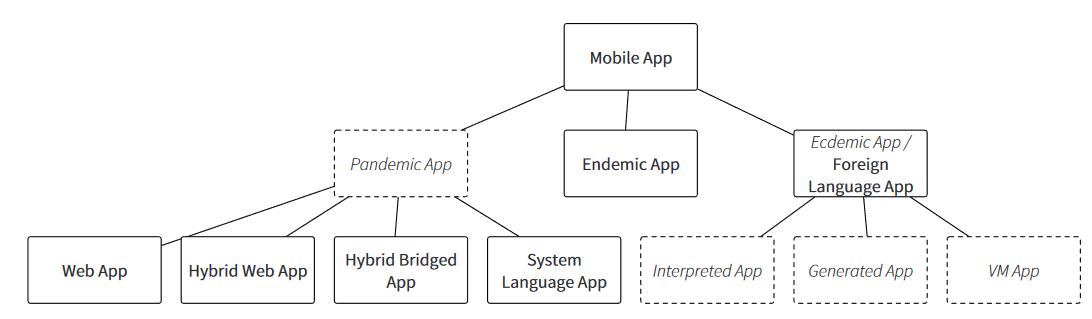
\includegraphics[width=0.9\textwidth]{Nunkesser_Hierarchy.png}
    \caption{Hierarchische Taxonomie der Entwicklungsansätze mobiler Apps \cite{Nunkesser_Taxonomy_Apps}.}
    \label{fig:Native_vs_CrossPlatform}
\end{figure}

Für den Zweck dieser Arbeit wird in den folgenden Abschnitten vorwiegend die übergreifende Kategorie der der Cross-Plattform Apps verwendet.
Diese umfasst die \textit{Hybrid Web Apps}, \textit{Hybrid Bridged Apps} und Foreign Language Apps.
Demnach wird im Folgenden zwischen Native-Apps beziehungsweise Endemic Apps, Web-Apps und Cross-Plattform Apps unterschieden.
Bei der Erläuterung der verschiedenen Frameworks wird dennoch eine Einordnung des jeweiligen Frameworks in eine Kategorie, wie von Nunkesser definiert, vorgenommen.
So können Vergleiche nicht nur zwischen einzelnen Frameworks, sondern auch zwischen verschiedenen Kategorien durchgeführt werden.
Die von Nunkesser als \textit{System Language Apps} bezeichnete Kategorie wird im Rahmen dieser Arbeit nicht zur Cross-Plattform Kategorie zugeordnet.
Bei System Language Apps erfolgt eine starke Bindung an das jeweilige \ac{SDK}, was die Wiederverwendung von Code sehr schwierig macht.
Bei geeigneter Architektur der App ist es hier jedoch möglich, Teile des Codes Systemübergreifend zu verwenden.
Für die Untersuchung von Frameworks für die Plattformübergreifende Entwicklung spielt dieser Ansatz aufgrund fehlender populärer Frameworks keine Rolle.
Außerdem ist die Bedeutung dieses Ansatzes für die Entwicklung mobiler Anwendungen in der Praxis allgemein vergleichsweise gering \cite{Nunkesser_Taxonomy_Apps}.

Obwohl sich die Ansätze der verschiedenen Kategorien, die hier als Cross-Plattform zusammengefasst werden, stark voneinander unterscheiden, weisen sie dennoch genügend Gemeinsamkeiten auf, die diese Zusammenfassung rechtfertigen.
Im Folgenden soll die Bezeichnung Cross-Plattform, jeweils als ein Ansatz verstanden werden, der die Wiederverwendung von Code, insbesondere zwischen den beiden mobilen Plattformen Android und iOS, fördert.
Gefordert wird zusätzlich die Möglichkeit, auf native Gerätefunktionen, wie Gerätesensoren oder die Kamera, zuzugreifen.
Es wird für die Kategorisierung nicht gefordert, dass der komplette Code wiederverwendet werden kann.


\subsection{Vorteile von Cross-Plattform Entwicklung}
\label{sec:CrossPlattform_Vorteile}

Trotz der Unterschiede der verschiedenen Cross-Pattform Ansätze und einzelnen Frameworks, welche im Verlauf dieser Arbeit noch aufgezeigt werden, können einige gemeinsame Vor- und Nachteile des Cross-Plattform Ansatzes identifiziert werden.
Die wichtigsten Vorteile und auch Nachteile der Cross-Plattform Entwicklung im Vergleich zur nativen Entwicklung sind in \autoref{fig:Native_vs_CrossPlatform} tabellarisch aufgeführt.
\begin{figure}[H]
    \centering
    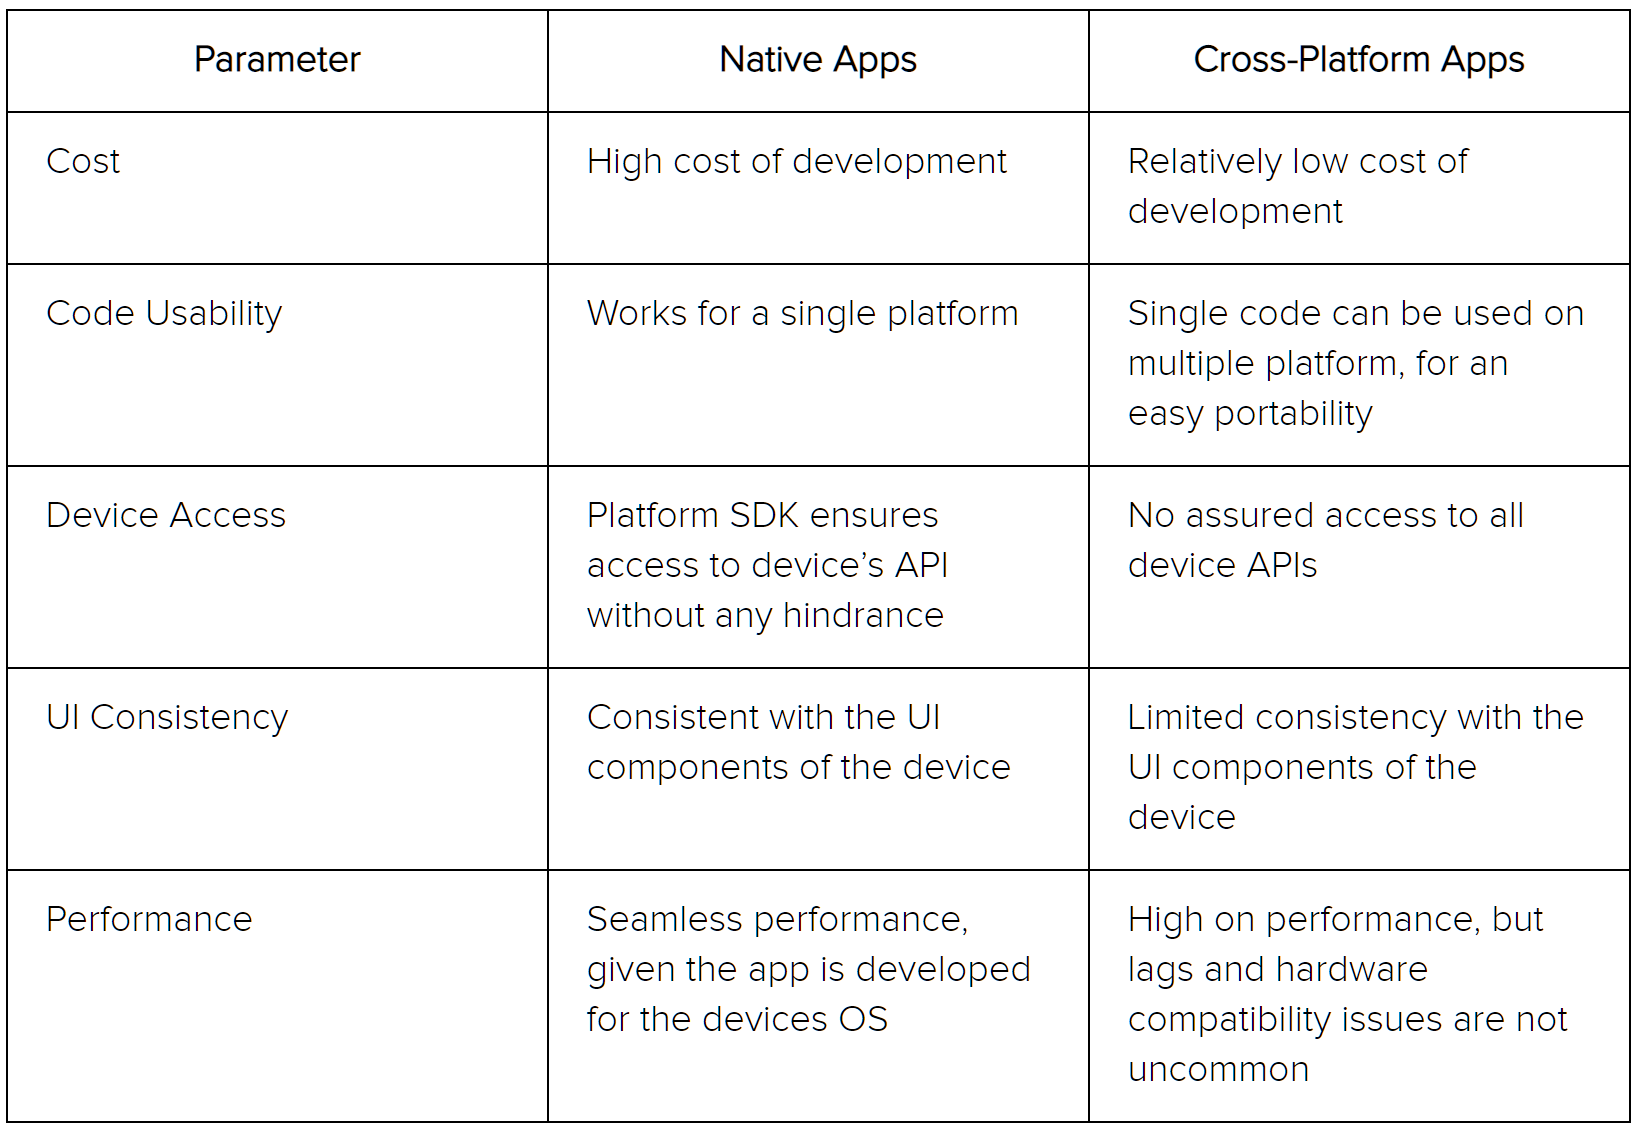
\includegraphics[width=0.9\textwidth]{Native_vs_CrossPlatform.png}
    \caption{Gegenüberstellung Entwicklungsansätze Native und Cross-Plattform \cite{Manchanda_CrossPlatformFrameworks}.}
    \label{fig:Native_vs_CrossPlatform}
\end{figure}

Alle Ansätze der teilen sich den Vorteil eines reduzierten Entwicklungsaufwands durch die einfache Wiederverwendung von Code.
Je nach verwendetem Framework kann der Anteil des geteilten Codes bis zu 100 \% betragen.
Allerdings ist es bei manchen Frameworks notwendig einzelne Funktionen in der jeweils nativen Programmiersprache zu implementieren.
Allgemein kann jedoch der überwiegende Teil des Codes wiederverwendet werden \cite{Nawrocki_Comparison_Hybrid_Native_Frameworks}.
Damit lassen sich die Entwicklungskosten im Vergleich zu nativen Apps durch die Cross-Plattform Entwicklung teils deutlich senken.
Matt Kremer, Enterprise Product Manager für das Ionic-Framework, gibt an, dass bei der Verwendung des Ionic-Frameworks sowohl Zeitaufwände für initiale Entwicklung und spätere Weiterentwicklung als auch die Personalkosten pro Woche geringer sind als bei einer nativen Entwicklung.
In einem Beispiel demonstriert er, wie die Kosten eines Ionic-Projekts weniger als 30 \% der Kosten eines vergleichbaren nativen Projekts betragen können \cite{Kremer_IonicROI}.
Hier ist jedoch zu bedenken, dass diese Angaben nicht durch eine unabhängige Quelle bestätigt wurden.
Dennoch sind sowohl Framework-Entwickler \cite{Xamarin_Einfuehrung, Kremer_IonicROI} als auch unabhängige Literatur \cite{Pinto_Native_to_Cross_Platform, Que_Comparison_Hybrid_Native, Nawrocki_Comparison_Hybrid_Native_Frameworks} einig, dass eine Cross-Plattform Entwicklung Kostenvorteile mit sich bringt.

Allgemeine Probleme gibt es beim Zugriff auf native \acp{API} der Geräte.
Einige Frameworks bieten direkten Zugriff auf einige native \acp{API}, andere setzen für jeglichen Zugriff auf Plugin-Systeme \cite{Heitkoetter_CrossPlatform_Comparison, Sasidaran_Survey_NativeHybrid}.
Meist können in einer Cross-Plattform App jedoch nicht alle nativ zur Verfügung stehenden Schnittstellen verwendet werden \cite{Pinto_Native_to_Cross_Platform}.

Auch bei der Konsistenz der Benutzeroberflächen schneiden die Cross-Plattform Ansätze meist schlechter ab als die native Entwicklung \cite{Manchanda_CrossPlatformFrameworks}.
Allerdings gibt es hier starke Unterschiede zwischen den Frameworks. 
Zum Beispiel verwendet ReactNative jeweils native \ac{UI}-Elemente, sodass die Benutzeroberfläche dem Look-and-Feel der Plattform entspricht \cite{React_NativeComponents}.

Ein gemeinsamer Nachteil aller Cross-Plattform Ansätze ist die durchschnittlich geringere Performance im Vergleich zu nativen Anwendungen \cite{Que_Comparison_Hybrid_Native, Pinto_Native_to_Cross_Platform}.
Einzelne Frameworks können für bestimmte Anwendungszwecke besser geeignet sein und andere können bei Betrachtung anderer Performancemetriken besser abschneiden.
Allgemein ist die Bewertung der Performance eines Frameworks immer vom Anwendungsfall und von der konkreten App abhängig.
In der Literatur finden sich verschiedene Untersuchungen \cite{Nawrocki_Comparison_Hybrid_Native_Frameworks,Biorn-Hansen_PerformanceOverhead_CrossPlatform,Jia_Performance}, welche sich mit der Performance von verschiedenen Cross-Plattform Frameworks beschäftigen. 
In keiner dieser Arbeiten wird jedoch die Performance für den konkreten Anwendungsfall der Videoaufzeichnung ausführlich untersucht.
\chapter{Populäre Cross-Plattform Frameworks}
\label{ch:Frameworks}

Im Folgenden sollen die vier populärsten Frameworks für die Cross-Plattform Entwicklung näher betrachtet werden.
Dabei liegt der Fokus auf der Funktionsweise der Frameworks und der Einordnung in eine der Kategorien nach Nunkesser, welche in \autoref{sec:Entwicklungsansaetze} vorgestellt wurden.
Bevor auf einzelne Frameworks eingegangen werden kann, müssen zunächst die aktuell populärsten Frameworks identifiziert werden.
Dazu werden insbesondere die StackOverflow Developer Surveys \cite{Stackoverflow_2020} \cite{Stackoverflow_2021} \cite{Stackoverflow_2022} der letzten Jahre herangezogen, welche Entwickler unter anderem zu ihren bevorzugten und im professionellen Bereich eingesetzten Frameworks befragen.
Diese Frameworks müssen im nächsten Schritt auf ihre Cross-Plattformfähigkeit hin untersucht werden.
Weiterhin wird auf die Umfrage \cite{Statista_UsedCrossPlatformFrameworks} zurückgegriffen, welche die am häufigsten eingesetzten Cross-Plattfom Frameworks zwischen 2019 und 2021 ermittelt hat.

% Verlauf laut Statista bis 2021, jeweils mit Top 4 von Stackoverflow, Top 4 Stackoverflow 2022


% Erläuterung der einzelnen Frameworks
\chapter{Implementierung und Evaluation}
\label{ch:evaluation}

Zunächst beschreibt \autoref{sec:implementierung} die Implementierung des Prototyps zur Videoaufzeichnung mit den entsprechenden Frameworks und die Bewertung der Grundfunktionalität des jeweiligen Prototyps.
Alle Prototypen stehen unter \url{https://github.com/lukaspanni/cross-platform-evaluation} unter der MIT-Lizenz zur Verfügung.
Dabei wird erläutert, wie die einzelnen Komponenten des Prototyps implementiert werden und welche zusätzlichen Komponenten eingesetzt werden müssen, um die geforderte Funktionalität umzusetzen.
Die Frameworks verwenden verschiedene Bezeichnungen für eingebundene Komponenten von Drittanbietern.
Zur einheitlichen Beschreibung werden diese in den folgenden Abschnitten jeweils als Plugins bezeichnet.
Außerdem wird jeweils beschrieben, inwiefern die geforderte Grundfunktionalität umgesetzt werden kann und welche Einschränkungen, zum Beispiel bei der Einstellung der Parameter, existieren.
In \autoref{sec:evaluation_allgemein} werden anschließend die Ergebnisse der allgemeinen Evaluationen nach den, in \autoref{sec:kriterien} beschriebenen Kriterien, zusammengefasst.

Für die Evaluierung werden die Prototypen jeweils auf einem Android- und einem iOS-Gerät getestet.
Konkret werden ein Google Pixel 4a 5G mit Android 13 und ein iPhone XR mit iOS 16.1.1 verwendet. 

\section{Implementierung und Evaluation der Grundfunktionalität}
\label{sec:implementierung}

Insgesamt ist festzustellen, dass die Grundfunktionalität der Aufzeichnung von Videos mit allen untersuchten Frameworks mit vorhandenen Plugins umgesetzt werden kann.
Auch der Zugriff auf den Gerätespeicher zur Speicherung der Videos ist in allen Frameworks möglich.
Dabei ist jedoch aufgefallen, dass kein Framework plattformübergreifende Speicherpfade unterstützt.
Stattdessen muss für jede Plattform ein passender Pfad, angepasst an die jeweilige Dateisystemstruktur, erzeugt werden.
Erste Unterschiede zeigen sich bei der Wiedergabe aufgezeichneter Videos.
Diese ist in Ionic mit Cordova mit allen getesteten Plugins nicht möglich.

Welche Komponenten verwendet wurden, welche Probleme aufgetreten sind und welche Einstellmöglichkeiten für die Parameter bestehen ist in den Abschnitten \ref{sec:evaluation_flutter} bis \ref{sec:evaluation_reactnative} beschrieben.

\subsection{Implementierung mit Flutter}
\label{sec:evaluation_flutter}

Flutter bringt verschiedene Abstraktionen für den Zugriff auf native Funktionen standardmäßig mit.
Für den Zugriff auf Kamerafunktionen muss jedoch ein Plugin genutzt werden.
Plugins für Flutter und Dart werden in einem öffentlichen Repository unter \url{https://pub.dev} zur Verfügung gestellt.
Mit dem Plugin \textit{camera} \cite{Dart_Camera} ist ein vom Flutter-Team gepflegtes offizielles Plugin verfügbar. 
Über dieses Plugin ist die Aufzeichnung von Videos unter Android und iOS möglich und einige Parameter können angepasst werden.
Für die Speicherung ist kein zusätzliches Plugin notwendig, der Zugriff auf Gerätespeicher ist in Flutter bereits integriert.
Zur Wiedergabe der Videos wird das offizielle Video-Player-Plugin verwendet \cite{Dart_Video}.

Die erforderlichen Anforderungen, sowie die Wiedergabe von Videos, können somit mit Flutter vollständig umgesetzt werden.
Allerdings gibt es einige Einschränkungen bei den einstellbaren Parametern.
So sind weder Belichtungszeit noch ISO-Wert einstellbar, für die Belichtung kann nur ein Offset für die automatische Belichtungssteuerung gesetzt werden.
Zudem kann die Aktualisierung der automatischen Belichtungssteuerung gestoppt werden, die letzte automatische Einstellung bleibt dabei erhalten.
Diese Funktion ist auch als \ac{AEL} bekannt.
Der Fokus kann ebenfalls nicht komplett manuell gewählt werden, stattdessen lässt sich ein Punkt des Videos wählen, welcher vom Autofokussystem als Ausgangspunkt verwendet wird.
Für das Bildformat stehen bis zu fünf verschiedene Voreinstellungen zur Verfügung, wobei die Verfügbarkeit vom verwendeten Gerät abhängt.
Weißabgleich, Videocodec und Bildrate lassen sich ebenfalls nicht einstellen.
Außerdem konnte nicht jeder verfügbare Sensor des Android-Testsmartphones ausgewählt werden.
Da das iOS-Testgerät nur jeweils einen Sensor für die Front- und Rückkamera besitzt, konnte diese Einschränkung unter iOS nicht getestet werden.


\subsection{Implementierung mit Ionic und Cordova}
\label{sec:evaluation_ionic}

Allgemein erlaubt Cordova den Zugriff auf native Funktionen, wie die Videoaufzeichnung nur über Plugins.
Erste Quelle für bestehende Plugins ist bei Verwendung von Ionic als UI-Toolkit die Sammlung offiziell unterstützter und getesteter Plugins, die unter \url{https://ionicframework.com/docs/native/} bereitsteht.
Hier konnten drei Plugins identifiziert werden, welche den Zugriff auf Kamerafunktionen ermöglichen.
Das naheliegende Plugin \textit{cordova-plugin-camera} erlaubt nur die Aufzeichnung von Bildern \cite{Cordova_Camera}.
Das Plugin \textit{cordova-plugin-camera-preview} ermöglicht zwar die Aufzeichnung von Videos, jedoch ist diese Funktion nur auf Android-Geräten verfügbar \cite{Cordova_CameraPreview}.
Lediglich das Plugin \textit{cordova-plugin-media-capture} erlaubt die Aufzeichnung von Videos auf allen Plattformen \cite{Cordova_MediaCapture}.
Jedoch verwendet dieses Plugin eine vom Betriebssystem bereitgestellte Aufzeichnungsfunktion, sodass aus der App heraus nur das Videoaufzeichnungsfenster geöffnet werden kann.
Außerdem sind deshalb keinerlei Einstellungen der in \autoref{tab:parameter_support} aufgeführten Parameter möglich.
Auch außerhalb der offiziellen Sammlung von verifizierten Plugins konnten keine Plugins identifiziert werden, welche die Einstellung einiger Parameter unterstützen.

Die Speicherung aufgezeichneter Videos erfolgt ohne zu erkennende Einschränkungen über das offizielle Plugin \textit{cordova-plugin-file} \cite{Cordova_File}.
Die Wiedergabe der Videos hingegen konnte weder über das HTML-Video Element noch durch ein Plugin realisiert werden. 

Damit sind die erforderlichen Anforderungen zwar umgesetzt, jedoch werden keine der optionalen Anforderungen erfüllt.
Um die optionalen Anforderungen umzusetzen, müssten spezifische Plugins implementiert werden.
Dementsprechend ist die Implementierung einer Videoaufzeichnungsanwendung mit Ionic und Cordova nur stark eingeschränkt möglich.


\subsection{Implementierung mit Xamarin}
\label{sec:evaluation_xamarin}

Da Xamarin prinzipiell die Nutzung der nativen \acp{API} unterstützt, sind theoretisch alle Kamerafunktionen nutzbar.
Allerdings sollen im Rahmen dieser Arbeit nur die vorhandenen plattformübergreifenden Abstraktionen des Frameworks genutzt werden.
Standardmäßig werden Open-Source Komponenten für .NET-Anwendungen über den Paketmanager NuGet verwaltet und im Repository \url{https://nuget.org} bereitgestellt.
Dort sind auch die offiziellen Xamarin-Bibliotheken verfügbar.
Die offizielle Bibliothek \textit{Xamarin.Essentials} ermöglicht neben der Nutzung weiterer nativer Funktionen auch den Zugriff auf verschiedene Kamerafunktionen.
Die Kamera kann über eine stark vereinfachte \ac{API} der statischen Klasse \textit{MediaPicker} genutzt werden \cite{Xamarin_MediaPicker}.
Wie das, in der Implementierung mit Cordova eingesetzte Plugin, wird auch hier die Aufzeichnung von Videos über die vom Betriebssystem bereitgestellte Aufzeichnungsfunktion realisiert.
Deshalb ist auch bei Xamarin-Anwendungen die Aufzeichnung von Videos zwar möglich, jedoch können keine Parameter aus der Anwendung heraus angepasst werden.
Der Zugriff auf den Gerätespeicher ist wie bei Flutter ohne zusätzliche Abhängigkeiten möglich.
Die Wiedergabe der Videos ist über ein entsprechendes \ac{UI}-Element der offiziellen Bibliothek \textit{XamarinCommunityToolkit} \cite{Xamarin_CommunityToolkit} ohne Einschränkungen möglich.

Ohne Nutzung nativer \acp{API} können mit Xamarin nur die Anforderungen zur Aufzeichnung und Speicherung sowie zur Wiedergabe von Videos erfüllt werden.
Die optionale Einstellbarkeit der Parameter lässt sich mit den vorhandenen Bibliotheken nicht umsetzen.


\subsection{Implementierung mit React Native}
\label{sec:evaluation_reactnative}

Für React Native existiert keine eigenständige Quelle für Plugins.
Stattdessen wird der JavaScript-Paketmanager \textit{npm} und die Registry unter \url{https://npmjs.com} verwendet, um Plugins zu verwalten.
Für die Videoaufzeichnung mit React Native konnten zwei geeignete Plugins identifiziert werden.
Da das Plugin \textit{react-native-vision-camera} \cite{Vision_Camera} bei der Einstellung von Parametern mehr Flexibilität bietet als das Plugin \textit{expo-camera} \cite{Expo_Camera}, wurde dieses für die prototypische Implementierung ausgewählt.
Zur Speicherung und Wiedergabe der Videos müssen zusätzlich \textit{react-native-fs} \cite{ReactNative_FileSystem} respektive \textit{react-native-video} \cite{ReactNative_Video} eingebunden werden.

Das Plugin \textit{react-native-vision-camera} verwendet die neue Architektur von React Native, wie in \autoref{sec:frameorks_reactnative} beschrieben.
Die neue Architektur ist bei neuen Projekten standardmäßig aktiviert und verwendet ohne weitere Konfiguration die JavaScript Engine Hermes.
Diese Einstellungen werden für die Implementierung beibehalten.

Die erforderlichen Anforderungen und die Wiedergabe von Videos können mit React Native ohne Einschränkungen umgesetzt werden.
Bei der Einstellbarkeit der Parameter gibt es im Vergleich mit den anderen Frameworks zudem weniger Einschränkungen.
So lässt sich beispielsweise der Sensor ohne Einschränkungen frei wählen.
Abhängig von den Fähigkeiten des Sensors werden die verfügbaren Einstellungen durch das Framework eingeschränkt.
Allgemein lassen sich die möglichen Einstellungen nach der Wahl des Sensors über das Plugin abfragen und können dem Nutzer angezeigt werden.
Verschiedene Sensoren unterstützen dabei unterschiedliche Kombinationen von Einstellungen, welche als Format bezeichnet werden.
Ein Format definiert dabei insbesondere das Bildformat und den verwendeten Farbraum.
Abhängig vom Format ist auch der Bereich, in welchem die Bildrate eingestellt werden kann.
Bei den Testgeräten war die Einstellung jeweils im Bereich von einem bis 60 Bildern pro Sekunde möglich.
Weiterhin kann der Fokus in ähnlicher Art und Weise wie bei Flutter gesetzt werden.
Im Vergleich zu Flutter kann jedoch die Belichtung nicht eingestellt werden.
Das Plugin erlaubt unter iOS zudem die Wahl des Videocodecs.
Dabei sind verschiedene Einschränkungen aufgefallen.
Beim Testgerät waren nur die Codecs H.264 und \ac{HEVC} und JPEG verfügbar.
Weiterhin war die Auswahl nur bei Auflösungen unter 3840x2160 möglich.
Diese und alle höheren Auflösungen unterstützen nur den Codec \ac{HEVC}.
Laut Dokumentation unterstützt das Plugin auch den Apple-eigenen Codec \textit{ProRes}, der aktuell allerdings nur auf den jeweiligen Pro-Modellen der iPhones 13 und 14 verfügbar ist \cite{Prores_iPhone13}.
Das Plugin bietet keine Möglichkeit die Belichtungsparameter ISO und Belichtungszeit einzustellen.

\subsection{Zusammenfassung Evaluation Grundfunktionalität}

Die geforderten Grundfunktionalitäten der Aufzeichnung und Speicherung können mit allen Frameworks umgesetzt werden.
Die Wiedergabe ist mit Ausnahme von Ionic mit Cordova ebenfalls möglich.
Bei der Einstellbarkeit der Parameter gibt es jedoch Unterschiede zwischen den Frameworks.
Insbesondere sind bei Xamarin und Ionic mit Cordova aufgrund der Nutzung der Standardanwendung zur Videoaufzeichnung keine Einstellungen der Parameter möglich.
Da Flutter und React Native die Standardanwendung nicht nutzen, sondern direkt die \acp{API} des Betriebssystems nutzen sind hier mehr Einstellungen möglich.
\autoref{tab:parameter_support_evaluation} fasst die Einstellbarkeit der Parameter für Flutter und React Native zusammen.
\begin{table}[H]
  \begin{tabularx}{\textwidth}{ |l|X|X| }
      \hline
      \textbf{Parameter} & \textbf{Flutter} & \textbf{React Native}  \\
      \Xhline{0.5mm}
      \textbf{Belichtungszeit} & \xmark & \xmark \\
      \hline
      \textbf{Sensorempfindlichkeit (ISO)} & \xmark & Wahl von Format mit unterschiedlichen Minimal- \& Maximalwerten \\
      \hline
      \textbf{Blende} & Über Sensor-Auswahl (Einschränkungen unter Android) & Über Sensor-Auswahl \\
      \hline
      \textbf{Brennweite} & Über Sensor-Auswahl (Einschränkungen unter Android) & Über Sensor-Auswahl \\
      \hline
      \textbf{Fokus} & Ausgangspunkt für Autofokussystem wählbar & Ausgangspunkt für Autofokussystem wählbar \\
      \hline
      \textbf{Weißabgleich} & \xmark & \xmark \\
      \hline
      \textbf{Bildrate} & \xmark & Bereich abhängig von Sensor und Format (Auflösung \& Farbraum) \\
      \hline
      \textbf{Bildformat} & Wahl aus maximal fünf Voreinstellungen & Wahl aus vom Gerät bereitgestellten Formaten (in Tests jeweils mehr Formate als Flutter) \\
      \hline
      \textbf{Kompressionsverfahren/Codec} & \xmark & nur unter iOS und abhängig von Auflösung \\
      \hline
  \end{tabularx}
  \caption{Einstellbarkeit der Parameter durch die Plugins für Flutter und React Native.}
  \label{tab:parameter_support_evaluation}
\end{table}






\section{Vergleich allgemeiner Kriterien}
\label{sec:evaluation_allgemein}

Im Folgenden werden die Ergebnisse der Evaluierung der Frameworks hinsichtlich der allgemeinen Kriterien zusammengefasst.
Dabei werden die Größe eines Release-Builds, die Zeit von Start der App bis zur vollständigen Funktionsfähigkeit und die zusätzlich benötigte Zeit für den definierten Ende-zu-Ende-Test betrachtet.

Da die Hardware der Testgeräte sehr unterschiedlich ist, sind die Ergebnisse nur eingeschränkt Plattformübergreifend vergleichbar.
Zum Beispiel ist das Android-Testgerät mit der doppelten Menge Arbeitsspeicher ausgestattet, verwendet jedoch einen, in synthetischen Benchmarks, langsameren Prozessor \cite{Comparison_Phones}.
Deshalb werden zusätzlich die auf die Mittelwerte der jeweiligen Plattformen normalisierten Werte betrachtet.
Da kein Android-Gerät mit der gleichen Hardware wie ein iOS-Gerät existiert, ist ein direkter Vergleich ohne Hardwareunterschiede nicht möglich.


\subsection{Größe eines Release-Builds}

Die jeweiligen Größen der Release-Builds in Mega-Byte sind in \autoref{fig:app_size} dargestellt.
Wie erwartet gibt es große Unterschiede abhängig vom verwendeten Framework.
Weiterhin fällt auf, dass iOS-Apps durchschnittlich größer sind als Android-Apps.
\begin{figure}[ht]
  \centering 
  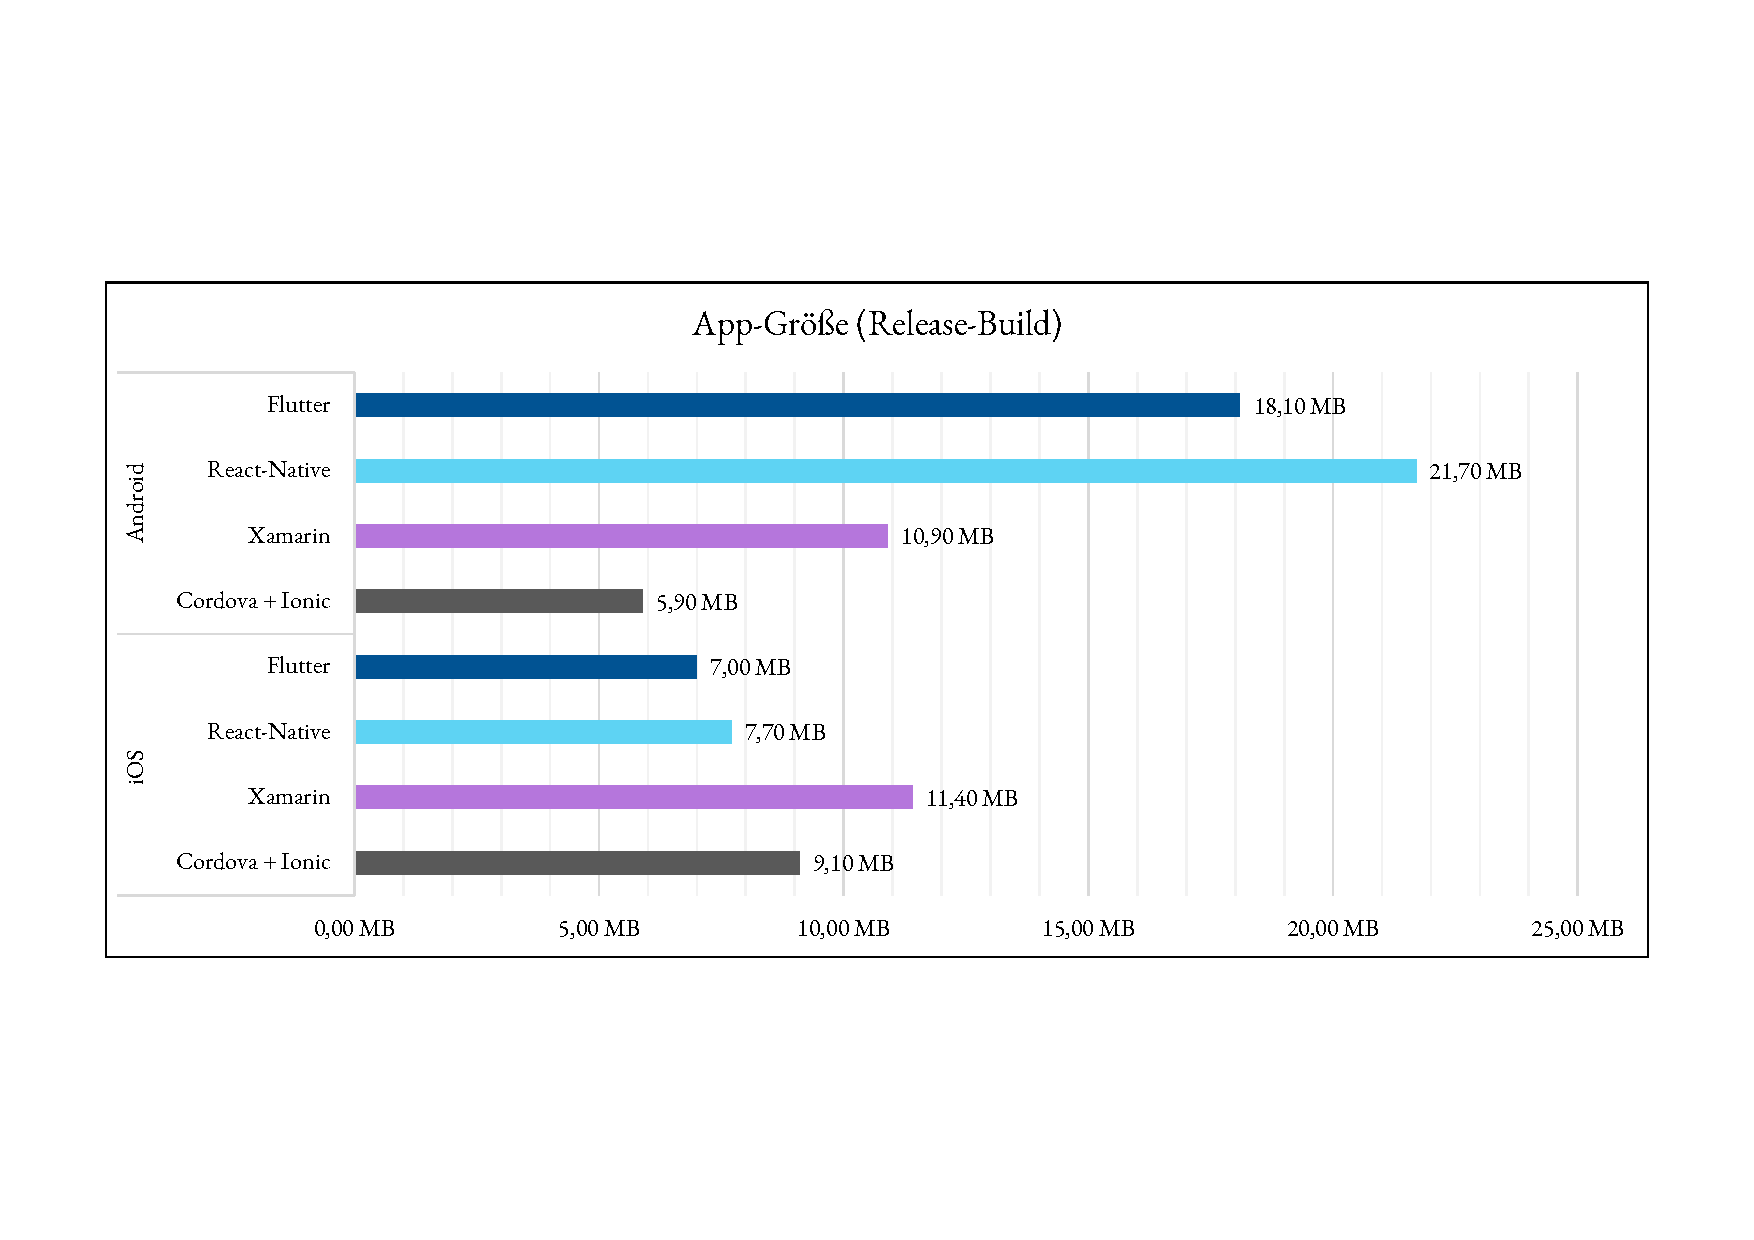
\includegraphics[trim=1.5cm 4.5cm 1.5cm 4.5cm, clip, width=0.9\textwidth]{app_size.pdf}
  \caption{Vergleich der Größe eines Release-Builds abhängig von Framework und Betriebssystem.}
  \label{fig:app_size}
\end{figure}

Unter Android sind die Release-Builds, welche mit Ionic und Cordova beziehungsweise Xamarin erstellt wurden, mit 5,9 MB und 10,9 MB vergleichsweise klein.
Dies kann auf die Verwendung der vom Betriebssystem bereitgestellten Videoaufzeichnungsanwendung zurückgeführt werden.
Die Größe der App lässt sich reduzieren, indem die vom Betriebssystem bereitgestellte Anwendung aufgerufen wird, anstatt eine eigene Implementierung zu verwenden.
Die gleiche Argumentation lässt sich auch auf die jeweiligen Implementierungen für iOS übertragen.
Auch unter iOS ist die mit Ionic und Cordova erstellte App kleiner als die Apps der anderen Frameworks.
Die \ac{IPA}-Datei von Xamarin-Anwendungen ist jedoch, wie durch die \ac{AOT}-Kompilation erwartet, deutlich größer als die entsprechende \ac{AAB}-Datei


Die mit Flutter und React Native erstellten Apps sind unter Android mit 18,1 MB und 21,7 MB deutlich größer als die mit Ionic und Cordova und Xamarin implementierten Anwendungen.
Da diese nicht auf die Standardanwendung des Betriebssystems zurückgreifen, muss die Funktionalität der Videoaufzeichnung in der App enthalten sein.
Weiterhin liefern sowohl React Native als auch Flutter verschiedene sonstige Abhängigkeiten mit, welche die Größe der App erhöhen.
Wie bei der Erläuterung der Frameworks in \autoref{sec:frameworks_flutter} beschrieben wird mit jeder Flutter-Anwendung eine Version der Skia Engine mitgeliefert.
Bei React Native muss jeweils eine JavaScript Engine mitgeliefert werden, in diesem Fall wird die für React Native optimierte Engine Hermes verwendet.

Unter iOS ist die mit React Native erstellte App mit 157,6 MB deutlich größer als alle anderen Anwendungen unabhängig vom Betriebssystem.
Zwar ist die App unter Android ebenfalls vergleichsweise groß, jedoch fällt der Unterschied weniger stark aus.
Sehr große \ac{IPA}-Dateien wurden bei der Verwendung der Hermes Engine bereits mehrfach beobachtet \cite{Hermes_appsize,Hermes_appsize_2}.
Wird anstatt Hermes, die von iOS bereitgestellte JavaScript Core Engine verwendet reduziert sich die App-Größe deutlich auf 3,1 MB, wie in \autoref{fig:reactnative_appsize_ios} zu sehen ist.
Unter Android trägt die Hermes Engine stattdessen zu einer kleineren App-Größe bei.
Ein Build mit der JavaScript Core Engine ist unter Android mit 51,9 MB deutlich größer als der Build mit der Hermes Engine mit 21,7 MB.
Da die Hermes Engine bei neuen React Native Projekten standardmäßig aktiviert ist, wird diese Variante für die Evaluation verwendet.
Außerdem ist anzumerken, dass die \ac{IPA}-Größe nicht repräsentativ für die Größe der App ist, welche über den App-Store verteilt wird.
Dies liegt daran, dass die \ac{IPA}-Datei verschiedene Varianten des Codes für verschiedene Geräte enthält und die finale, optimierte Version der App erst beim Upload zum App-Store erstellt wird \cite{IPA_Size}.
Da jedoch keine Methode bekannt ist, mit der die finale App-Größe bestimmt werden kann, ohne ein kostenpflichtiges Entwicklerkonto bei Apple zu besitzen, muss die \ac{IPA}-Größe zur Bewertung verwendet werden.

\begin{figure}[ht]
  \centering 
  
\includegraphics[clip, width=0.9\textwidth]{reactnative_appsize_ios}
   \caption{Vergleich der App-Größe einer React Native Anwendung für iOS mit und ohne Verwendung der Hermes Engine.}
  \label{fig:reactnative_appsize_ios}
\end{figure}


\subsection{Dauer bis zur vollständigen Funktionsfähigkeit}

Wie lange die jeweiligen Apps zwischen Start und vollständiger Funktionsfähigkeit benötigen, ist in \autoref{fig:launch_time} dargestellt.
Jeder Wert ist dabei als Mittelwert aus fünf Messungen angegeben.
Nach jeder Messung wurde die App komplett beendet, damit Kaltstartzeiten gemessen werden können.

Unter Android sind alle Startzeiten konsistent zwischen 50 und 64 \% schneller als unter iOS.
Dies kann vermutlich auf Hardwareunterschiede und Unterschiede im Betriebssystem zurückgeführt werden.
Insbesondere die große Differenz der verfügbaren Arbeitsspeichermenge könnte hier eine Rolle spielen.
Die auf die durchschnittliche Startzeit auf dem jeweiligen Testgerät normalisierten Zeiten sind in \autoref{fig:launch_time_normalized} dargestellt.
Hier fallen kaum Unterschiede zwischen den Plattformen auf, was die Vermutung bekräftigt, dass die Unterschiede auf grundsätzliche Unterschiede der Hardware und der Betriebssysteme zurückzuführen sind.
\begin{figure}[ht]
  \centering 
  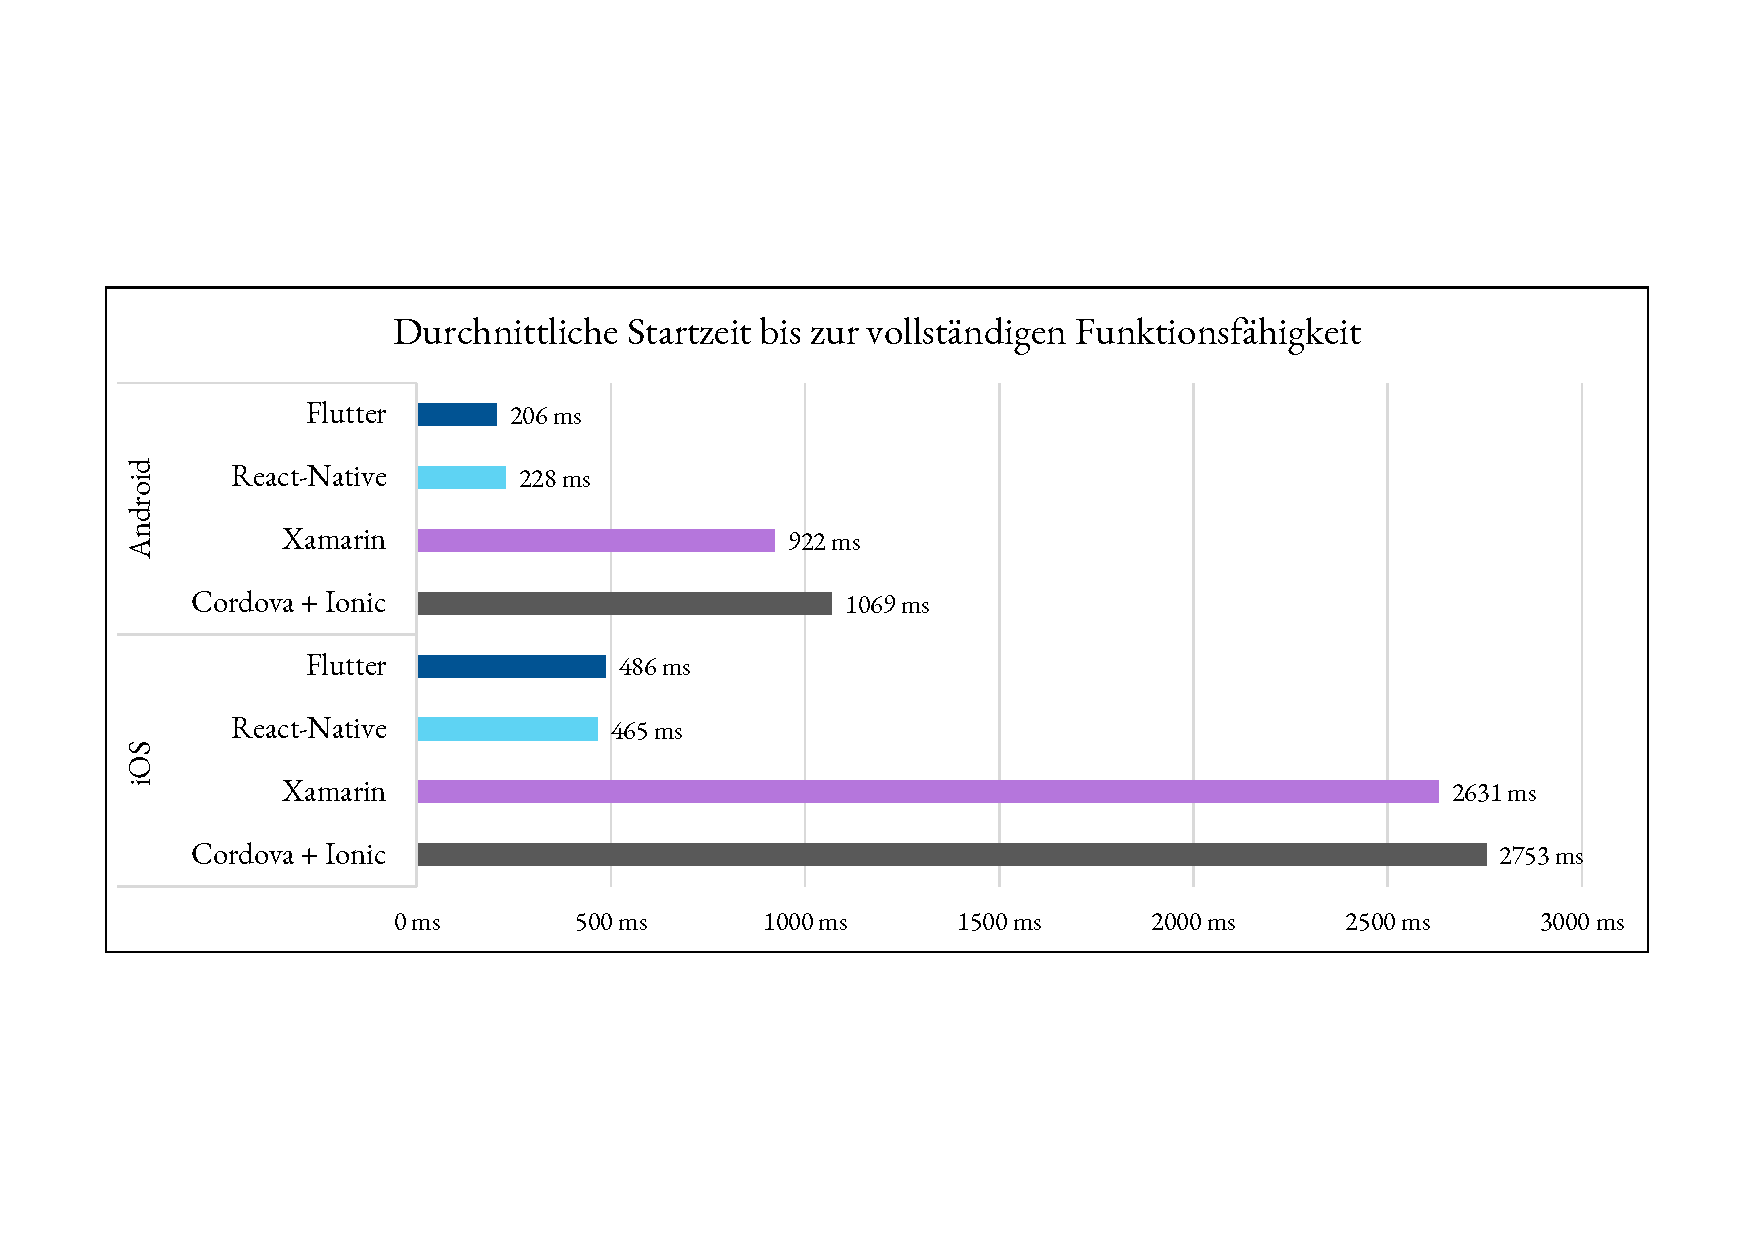
\includegraphics[trim=1.8cm 4.5cm 1.8cm 4.5cm, clip, width=0.9\textwidth]{launch_time.pdf}
  \caption{Vergleich der Zeit bis zur vollständigen Funktionsfähigkeit des Prototyps abhängig von Framework und Betriebssystem.}
  \label{fig:launch_time}
\end{figure}


Für die Messung der Startzeit kann bei Flutter und Xamarin auf die \ac{TTFD} zurückgegriffen werden, die bei diesen Frameworks der Zeit bis zur vollständigen Funktionsfähigkeit entspricht.
Andererseits kann die \ac{TTFD} bei React Native und Ionic mit Cordova nicht herangezogen werden, da diese Frameworks die Initialisierung nicht komplett abgeschlossen haben, wenn das erste Frame gerendert wird.
Bei Ionic mit Cordova kann die \ac{TTFD} nur bis zur Anzeige der Wrapper-Anwendung gemessen werden.
Die folgende Initialisierung der WebView mit der eigentlichen Anwendung in JavaScript kann nicht berücksichtigt werden.
Deshalb wird stattdessen die Zeit bis zum Event \texttt{Platform.ready} verwendet, welches ausgelöst wird, wenn die Anwendung komplett bereit ist.
Auch bei React Native ist die \ac{TTFD} nicht aussagekräftig, da auch hier die Initialisierung des Frameworks nicht mit der Initialisierung des nativen Teils abgeschlossen ist.
Ab dem ersten Aufruf der \texttt{render}-Methode kann beliebiger Code ausgeführt werden, weshalb dieser Zeitpunkt als Messzeitpunkt verwendet wird.

Von allen untersuchten Frameworks starten Flutter und React Native Anwendungen am schnellsten.
Unter Android ist Flutter dabei etwas schneller als React Native, unter iOS ist es umgekehrt.

\begin{figure}[ht]
  \centering 
  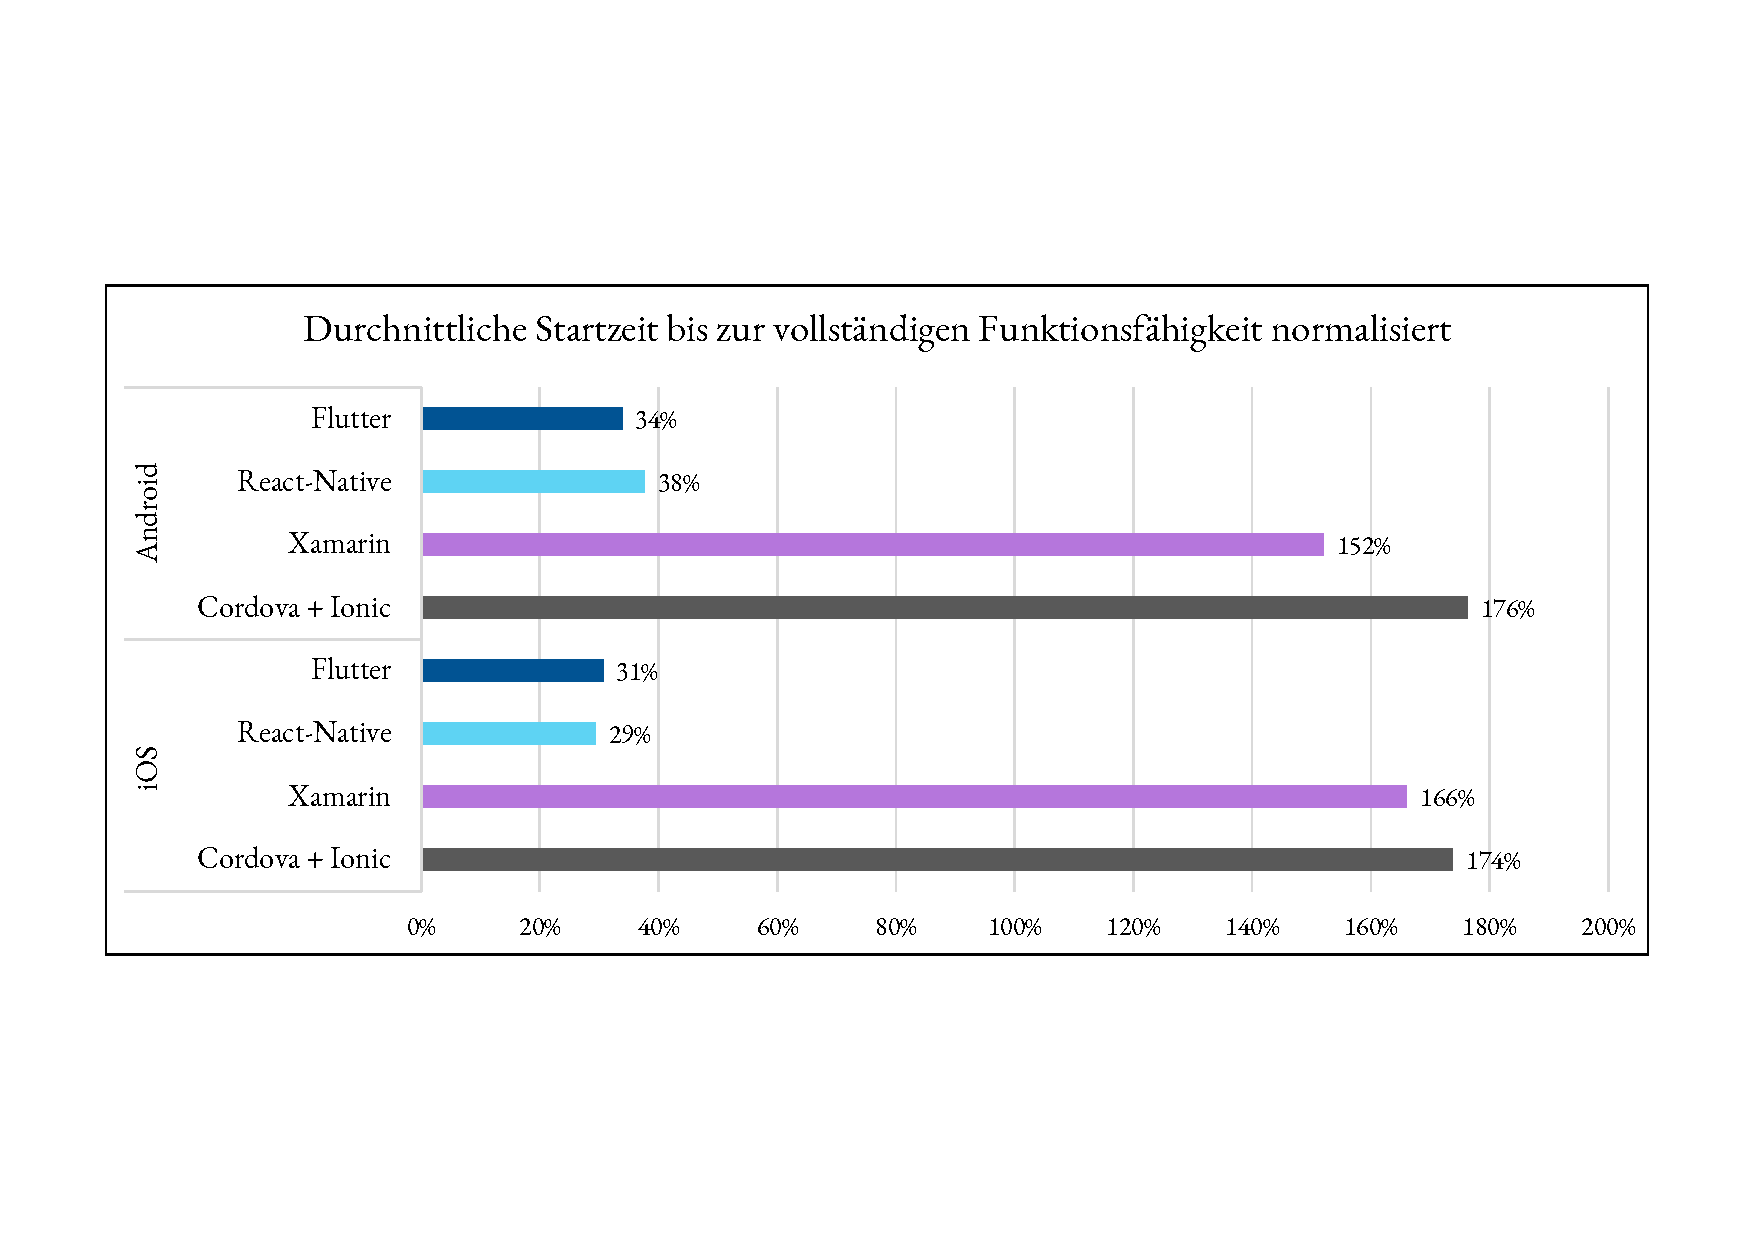
\includegraphics[trim=1.8cm 4.5cm 1.8cm 4.5cm, clip, width=0.9\textwidth]{launch_time_normalized.pdf}
  \caption{Vergleich der Zeit bis zur vollständigen Funktionsfähigkeit des Prototyps abhängig von Framework und Betriebssystem, normalisiert auf die durchschnittliche Startzeit des Geräts.}
  \label{fig:launch_time_normalized}
\end{figure}
Die Xamarin-Anwendung und die Anwendung, welche mit Ionic und Cordova implementiert ist, benötigen deutlich länger, bis die vollständige Funktionsfähigkeit erreicht ist.
Obwohl sowohl bei Ionic mit Cordova als auch bei React Native die Logik in JavaScript implementiert ist, ist die Startzeit der React Native-Anwendung mehr als viermal kürzer.
Daraus lässt sich schließen, dass der Ansatz von React Native, die nativen Steuerelemente der Plattform anstelle einer WebView einzusetzen, beim Starten der Anwendung einen deutlichen Vorteil bietet.
Allerdings nutzt React Native auch eine für das Framework optimierte JavaScript Engine, was vermutlich ebenfalls einen positiven Einfluss auf die Startzeit hat.

Für Xamarin-Anwendungen wurde aufgrund der \ac{JIT}-Kompilation unter Android eine deutlich längere Startzeit als unter iOS erwartet.
Mit 166 \% der durchschnittlichen Startzeit unter iOS und 152 \% der durchschnittlichen Startzeit unter Android fällt der Unterschied zwischen den beiden Plattformen jedoch weniger stark aus als angenommen.
Ein Grund dafür konnte nicht identifiziert werden.

\subsection{Ende-zu-Ende-Test}

Die automatisierte Aufzeichnung und Speicherung eines Videos für den Ende-zu-Ende-Test ist nur bei Flutter- und React Native-Anwendungen möglich.
Sowohl bei Ionic mit Cordova als auch bei Xamarin kann die Aufzeichnung von Videos aufgrund der Verwendung der Standardanwendung zur Videoaufzeichnung nicht automatisiert werden.
Die in \autoref{fig:testcase} aufgeführten Zeiten, stellen jeweils einen Mittelwert aus fünf Messungen dar.
Für die Messung wurden dabei die von den Frameworks bereitgestellten Funktionen zur Zeitmessung verwendet.
Vom gemessenen Wert wird zusätzlich die Dauer des aufgezeichneten Videos abgezogen, da diese in allen Tests gleich gesetzt wurde.

\begin{figure}[ht]
  \centering 
  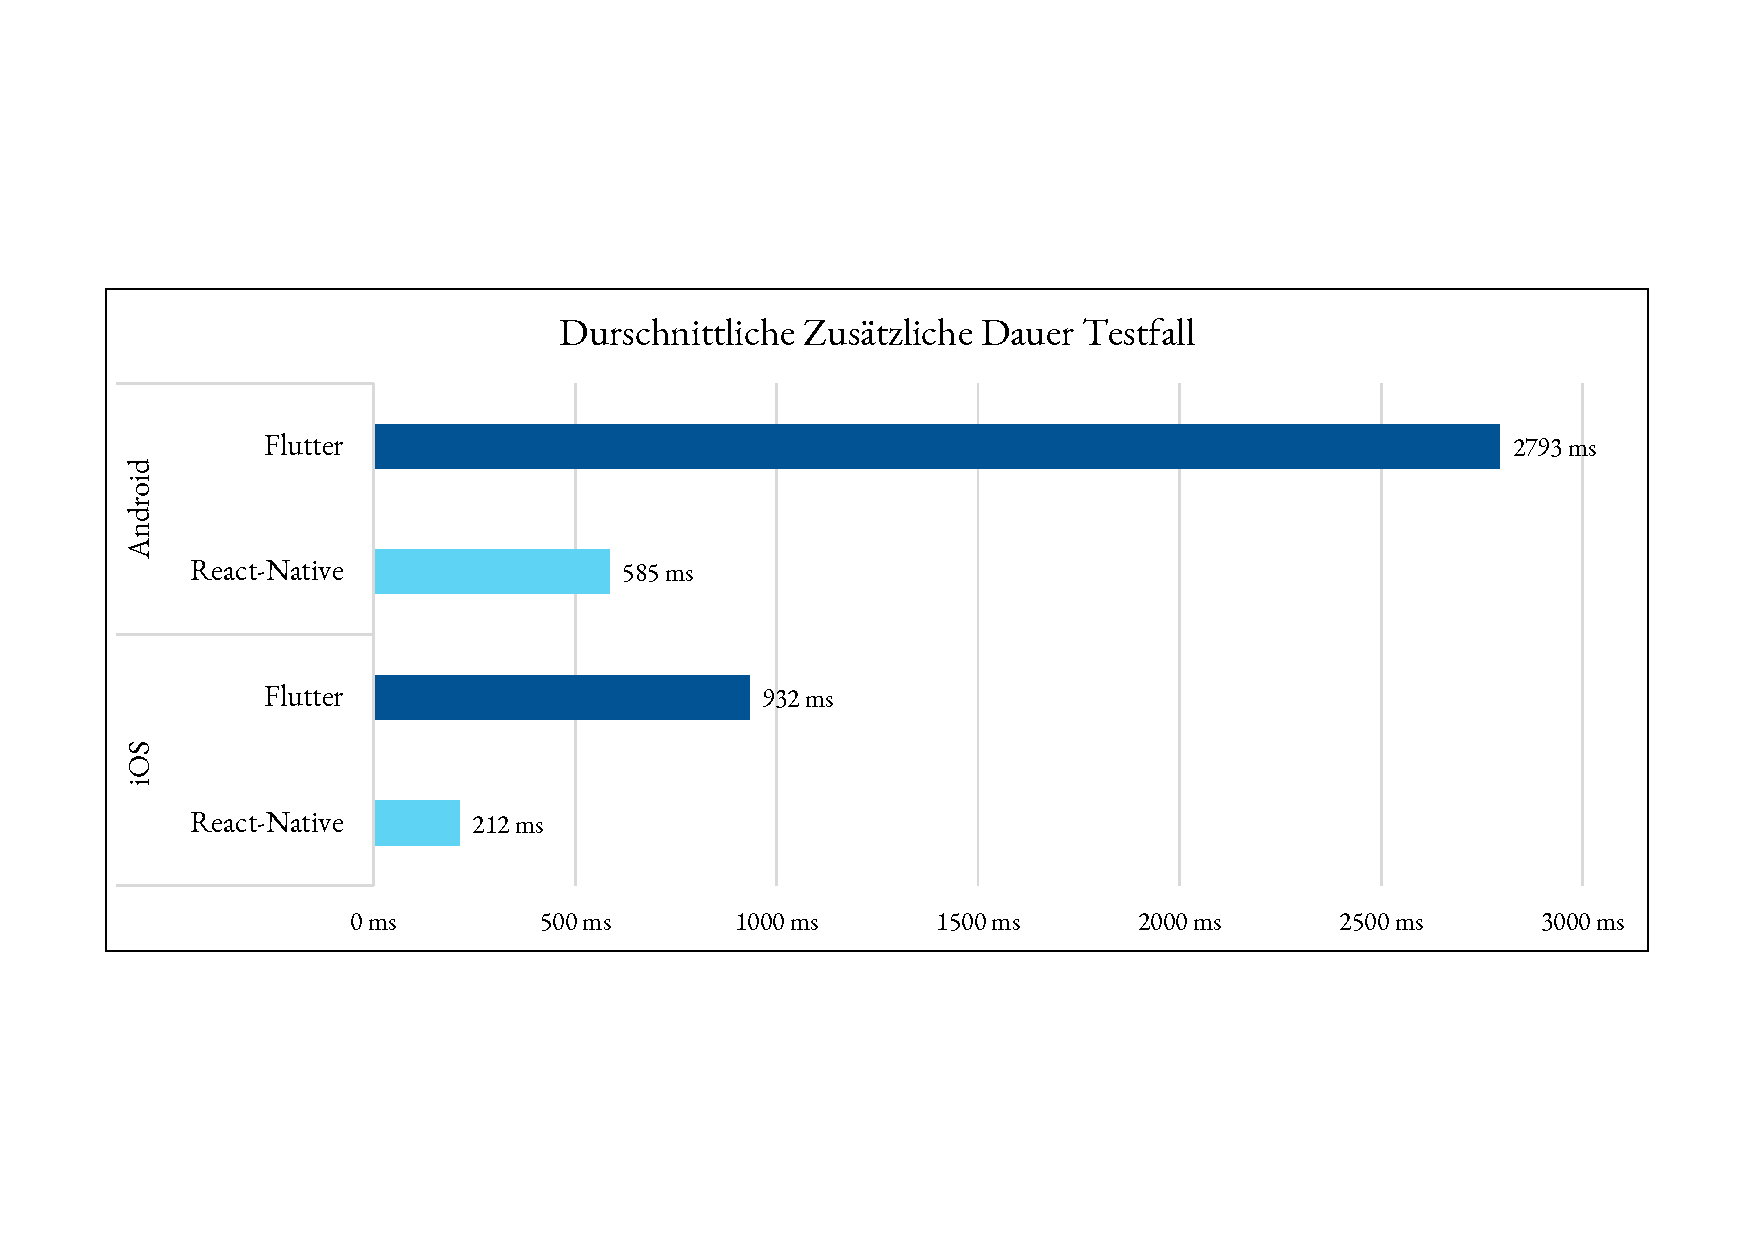
\includegraphics[trim=1.8cm 4.5cm 1.8cm 4.5cm, clip, width=0.9\textwidth]{testcase.pdf}
  \caption{Vergleich der für die Aufzeichnung und Speicherung von zehn Sekunden Video zusätzlich benötigten Zeit abhängig von Framework und Betriebssystem.}
  \label{fig:testcase}
\end{figure}

Direkt auffällig ist, dass die zusätzlich benötigte Zeit unter iOS deutlich geringer ausfällt als unter Android.
Dies lässt sich vermutlich auf Unterschiede der verwendeten Hardware und grundsätzliche Unterschiede zwischen den Betriebssystemen zurückführen.
Es wird angenommen, dass der Overhead für den Zugriff auf Kamerafunktionen und den Gerätespeicher unter iOS geringer ist als unter Android.
Außerdem kann der performantere Prozessor des iOS-Testgeräts, insbesondere bei der aufwändigen Codierung des Videos, zu einer schnelleren Ausführung beitragen.

\begin{figure}[ht]
  \centering 
  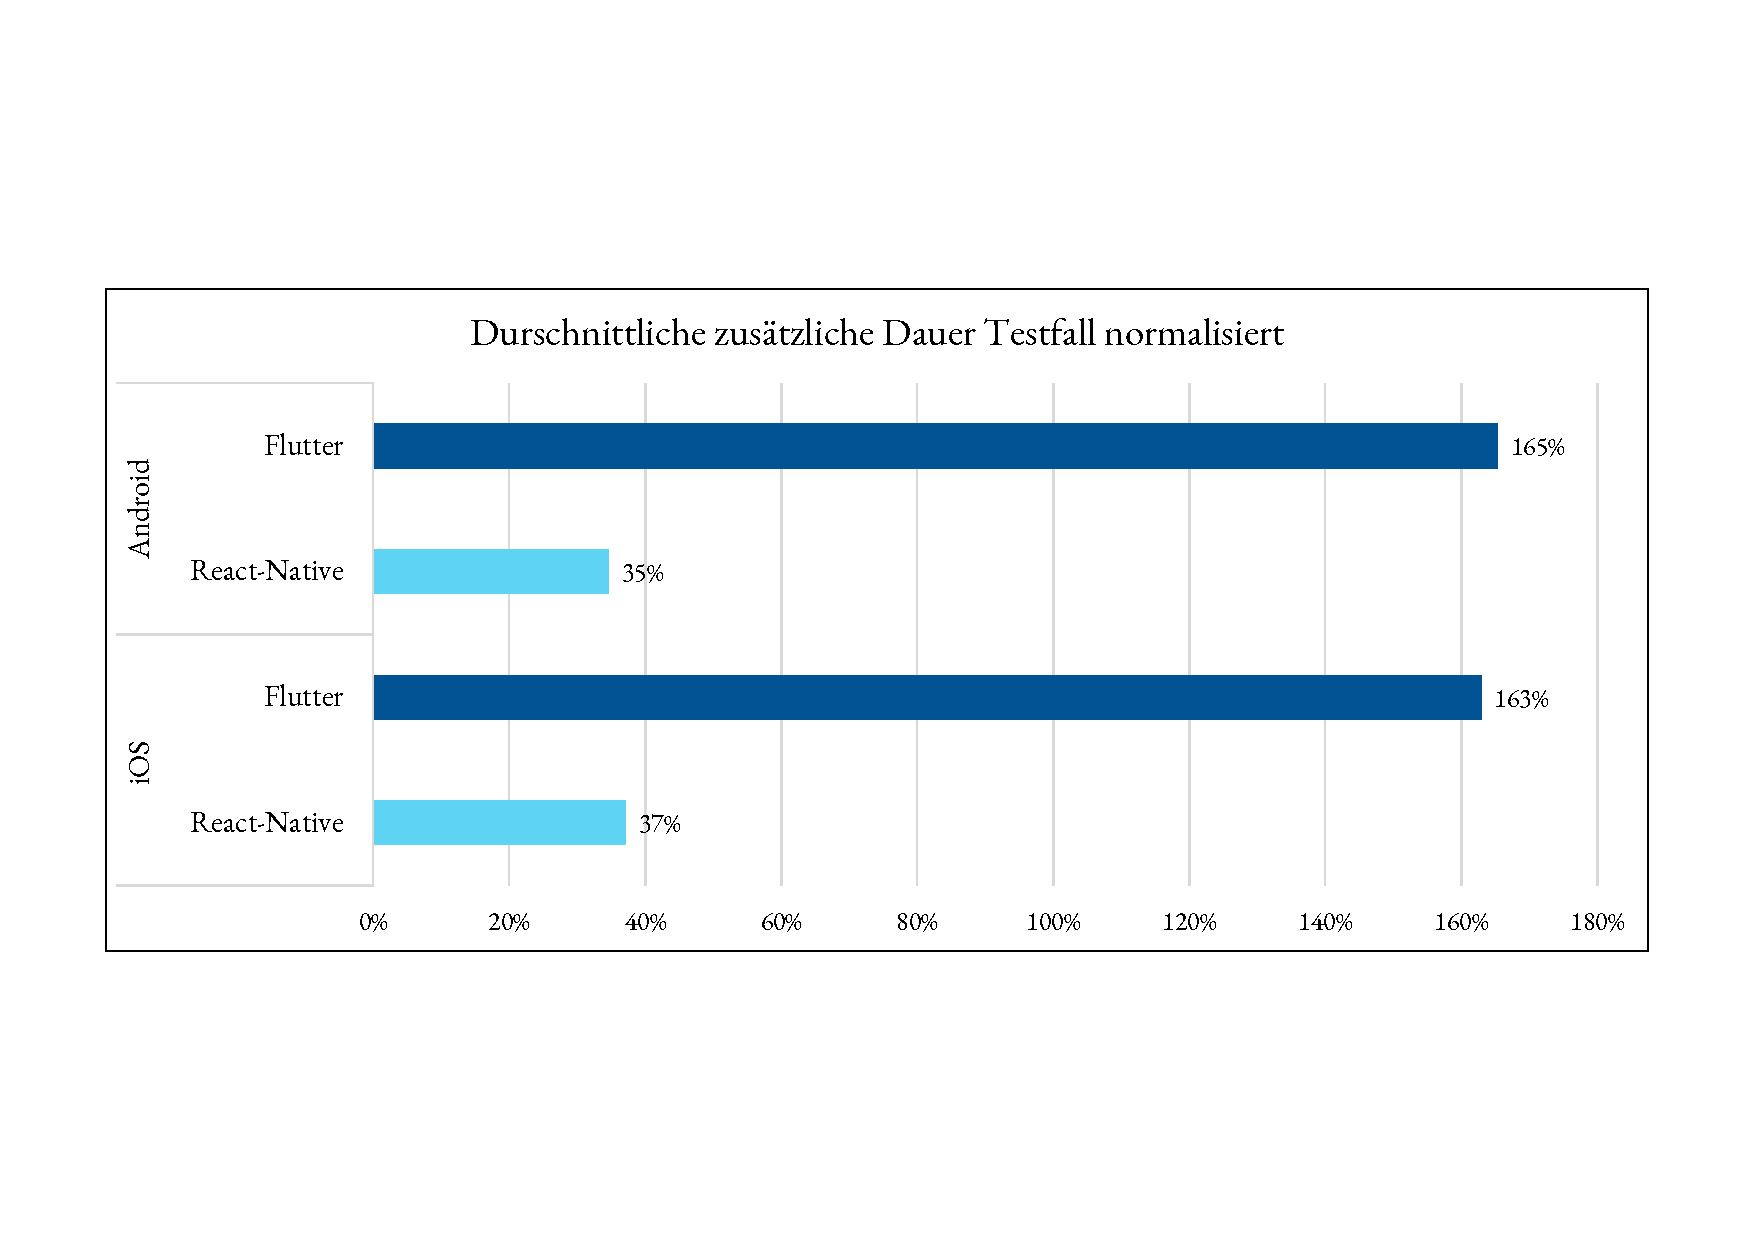
\includegraphics[trim=1.8cm 4.5cm 1.8cm 4.5cm, clip, width=0.9\textwidth]{testcase_normalized.pdf}
  \caption{Vergleich der für die Aufzeichnung und Speicherung von zehn Sekunden Video zusätzlich benötigten Zeit, normalisiert auf die durchschnittliche Zeit.}
  \label{fig:testcase_normalized}
\end{figure}
Die normalisierten Werte in \autoref{fig:testcase_normalized} zeigen, dass der Unterschied zwischen den Frameworks unter Android und iOS nahezu identisch ausfällt.
In beiden Fällen ist der automatisierte Testfall in der React Native-Anwendung mehr als viermal schneller als in der mit Flutter implementierten Anwendung.
Dies lässt sich mit fundamentalen Unterschiede zwischen den Frameworks erklären.
Beide Frameworks wählen zum Zugriff auf native Funktionen einen unterschiedlichen Ansatz.

Das eingesetzte React Native Plugin verwendet die neue, in \autoref{sec:frameorks_reactnative} beschriebene, Architektur.
Damit können plattformspezifische Host-Objects direkt aus JavaScript aufgerufen werden.
Dadurch entfällt insbesondere der Aufwand für Serialisierung und Deserialisierung von Nachrichten, welche zwischen dem nativen Teil und dem plattformübergreifenden Teil der Anwendung ausgetauscht werden müssen.
Im Vergleich verwenden sowohl die alte Architektur von React Native als auch die Architektur von Flutter eine Nachrichtenbasierte Kommunikation.
Somit erfordert jeder Funktionsaufruf zwei zusätzliche Nachrichten, welche jeweils eine Serialisierung und Deserialisierung erfordern.
Weiterhin verbergen die Plugins die nativen Aufrufe, sodass aus der Anwendung heraus nicht ersichtlich ist, wie viele native Funktionsaufrufe durch den Aufruf einer Plugin-Funktion ausgelöst werden.

Durch den grundsätzlich unterschiedlichen Ansatz beim Zugriff auf native Funktionen ist der effizientere Zugriff auf native Funktionen durch React Native vermutlich nicht auf die hier getesteten Funktionen beschränkt.


\subsection{Zusammenfassung Evaluation allgemeine Kriterien}

Mit einer kurzen Startzeit, der besten Performance beim Ende-zu-Ende-Test und der größten Freiheit bei der Einstellung der Video-Parameter ist React Native als am besten geeignetes Framework für die Entwicklung einer Videoaufzeichnungsanwendung für Android und iOS zu bewerten.
Zudem lässt sich das Problem der App-Größe unter iOS durch die Nutzung der JavaScriptCore Engine umgehen.
Nur Flutter ist ebenfalls als empfehlenswert zu bewerten.
Startzeiten sind sehr ähnlich zu React Native, allerdings fällt die Performance im Ende-zu-Ende-Test deutlich schlechter aus und weniger Parameter können eingestellt werden.
Weiterhin ist die App-Größe unter iOS deutlich und unter Android geringfügig kleiner.
Jedoch muss beachtet werden, dass die stark gestiegene App-Größe für React Native unter iOS als Fehler im Zusammenspiel mit der Hermes Engine zu betrachten ist.
Dennoch kommt die Flutter-Anwendung mit weniger Plugins aus, da der Zugriff auf das Dateisystem bereits in Flutter integriert ist.
Ionic mit Cordova und Xamarin eignen sich hingegen nur schlecht für die Umsetzung von Videoaufzeichnung.
Nicht nur die komplett fehlende Einstellbarkeit der Parameter, sondern auch mehr als viermal langsamere Startzeiten, schränken die Eignung stark ein. 

Diese Ergebnisse können als Begründung für die hohe Beliebtheit von Flutter und React Native im Vergleich zu Ionic mit Cordova und Xamarin dienen.
Jedoch können die Ergebnisse umgekehrt auch in der hohen Beliebtheit begründet sein.
Für den Zugriff auf die Kamerafunktionalität wurden jeweils zusätzliche Open-Source Plugins verwendet.
Bei einer größeren Beliebtheit unter Entwicklern ist davon auszugehen, dass sich mehr Entwickler an der Entwicklung von Open-Source Plugins beteiligen.
Damit steigt die Wahrscheinlichkeit, dass ein Plugin für die benötigte Funktionalität bereits existiert und die Qualität der Plugins sollte ebenfalls höher sein.
Andererseits sorgt eine geringe Beliebtheit, wie bei Ionic mit Cordova oder Xamarin dafür, dass sich wahrscheinlich weniger Entwickler an der Entwicklung von Open-Source Plugins beteiligen, wodurch weniger gute Plugins zur Verfügung stehen.
\chapter{Fazit}
\label{ch:fazit}


Cross-Plattform Frameworks können die Entwicklung von Apps für die beiden mobilen Plattformen Android und iOS deutlich erleichtern.
Während der klassische Ansatz die Entwicklung mit der, vom Betriebssystem vorgegebenen Programmiersprache vorsieht, ermöglichen Cross-Plattform Frameworks die überwiegende Verwendung einer gemeinsamen Programmiersprache.
So lässt sich ein großer Anteil des Codes für beide Plattformen wiederverwenden, was benötigte Zeit und Kosten für die Entwicklung deutlich reduziert.
Allerdings müssen Apps für viele Funktionen auf die \acp{API} des Betriebssystems zurückgreifen.
Da sich die \acp{API} der beiden Betriebssysteme teilweise stark unterscheiden ist plattformspezifischer Code notwendig.
Für häufig verwendete Funktionen existieren Abstraktionen der Frameworks oder entsprechende Plugins von Drittanbietern, sodass auch hier die Wiederverwendung von Code möglich ist.
Jedoch ist ein Plugin immer für einen bestimmten Anwendungsfall konzipiert und stellt eventuell nicht alle benötigten Funktionen und Einstellmöglichkeiten zur Verfügung.
Im Rahmen der vorliegenden Arbeit wurde untersucht, inwiefern der Anwendungsfall einer Videoaufzeichnung mit den vorhandenen Abstraktionen und Plugins der populärsten Cross-Plattform Frameworks umgesetzt werden kann.
Durch die verschiedenen Ansätze der Frameworks und die unterschiedliche Verfügbarkeit von Plugins konnten große Unterschiede in der Eignung der Frameworks festgestellt werden.


Die Frameworks Flutter, Cordova mit Ionic als UI-Toolkit, Xamarin und React Native wurden als populärste Cross-Plattform Frameworks identifiziert.
Bei Untersuchung der Funktionsweise in \autoref{ch:frameworks} wird klar, dass die Frameworks unterschiedliche Ansätze zur Umsetzung der plattformübergreifenden Entwicklung verfolgen.
Unterschiede bestehen nicht nur in der verwendeten Programmiersprache, sondern auch in der grundlegenden Architektur und der Art des Zugriffs auf native Funktionen.
Alle Frameworks ermöglichen jedoch prinzipiell den Zugriff auf alle \acp{API} der mobilen Betriebssysteme.
Nur mit Xamarin ist eine direkte Nutzung der Schnittstellen möglich, ohne für die jeweilige Plattform nativen Code entwickeln zu müssen.
Die anderen Frameworks setzen auf Plugin-Systeme.
Dabei steht eine Vielzahl von Plugins von den Frameworkentwicklern und von Drittanbietern als Open-Source-Software zur Verfügung, sodass viele Anwendungsfälle umsetzbar sein sollten.
Damit ist es mit jedem der untersuchten Frameworks grundsätzlich möglich, eine App zur Videoaufzeichnung zu entwickeln.


Für die Implementierung von prototypischen Apps wurde jeweils nur auf verfügbare Plugins oder Bibliotheken zurückgegriffen.
Keine Funktion wurde direkt in nativen Code umgesetzt.
Durch die Implementierung von speziellen Plugins in nativem Code ginge der Vorteil der Cross-Plattform Frameworks verloren.
Die essenziellen, funktionalen Anforderungen, definiert in \autoref{ch:bewertungskriterien}, konnten mit allen Frameworks umgesetzt werden.
Bei der Umsetzung der optionalen Anforderungen und der Untersuchung von Startzeit, App-Größe und Performance in einem Ende-zu-Ende-Test, wurden jedoch deutliche Unterschiede zwischen den Frameworks festgestellt.

React Native hat sich als am besten geeignetes Framework für die Entwicklung einer App zur Videoaufzeichnung beziehungsweise für Apps mit vielen nativen Zugriffen herausgestellt.
Mit keinem anderen Framework konnten mehr Parameter der Videoaufzeichnung auf die eigenen Bedürfnisse angepasst werden.
Dennoch sind nicht alle wünschenswerten Parameter verfügbar.
Außerdem ist die Performance des React Native Prototyps im Ende-zu-Ende-Test am besten.
Als Grund wurde die effiziente Kommunikation zwischen plattformübergreifenden und nativen Komponenten identifiziert.
Einziges Problem ist die sehr große App-Größe unter iOS, welche jedoch vermutlich auf einen Fehler im Zusammenspiel mit der JavaScript Engine Hermes zurückzuführen ist.
Nur Flutter wird als weiters Framework für die Entwicklung einer App zur Videoaufzeichnung empfohlen.
Die Einstellbarkeit der Parameter für die Videoaufzeichnung ist jedoch bei dem für Flutter verwendeten Plugin nicht so umfangreich wie bei React Native.

Die Verfügbarkeit von Plugins, welche für den konkreten Anwendungsfall gut geeignet sind, konnte allgemein als entscheidendes Kriterium für die Eignung eines Frameworks identifiziert werden.
Da für Cordova und Xamarin keine Plugins existieren, welche den Anwendungsfall der Videoaufzeichnung gut unterstützen, werden diese Frameworks nicht empfohlen.
Technisch wäre die Umsetzung der Funktionalität in Form von Plugins für diese Frameworks ohne Einschränkungen möglich.
Als Grund für das Fehlen von Plugins wurde stattdessen die im Vergleich geringere Popularität und Verbreitung von Cordova und Xamarin identifiziert.
React Native und Flutter sind hingegen unter Entwicklern weit verbreitet und sehr beliebt.
Damit kann davon ausgegangen werden, dass diese Frameworks auch für andere Anwendungsfälle die besseren Plugins bieten.


Abschließend kann festgehalten werden, dass zur Entwicklung einer App zur Videoaufzeichnung React Native und Flutter in Betracht gezogen werden können.
Jedoch lassen sich mit keinem der verfügbaren Plugins für die Frameworks, alle wünschenswerten Parameter für die Videoaufzeichnung einstellen.
Werden alle Parameter benötigt, müssen entweder die bestehenden Plugins erweitert werden oder die Entwicklung muss nativ erfolgen.
Sofern nicht alle der Parameter benötigt werden, kann die Nutzung der Cross-Plattform Frameworks allerdings eine deutliche Zeit- und Kostenersparnis bringen.


\section{Ausblick}

Die Ergebnisse dieser Arbeit können als Grundlage für die Untersuchung weiterer Anwendungsfälle dienen.
Wie in \autoref{ch:auswahl} beschrieben, wird davon ausgegangen, dass die Unterschiede zwischen den Frameworks bei Anwendungsfällen, die weniger native Funktionen nutzen, deutlich kleiner ausfallen.
Auf Basis der Untersuchung der App-Größe und der Startzeit wird für solche Anwendungsfälle Flutter empfohlen.
Diese Annahmen sollten in weiteren Untersuchungen überprüft werden.

Allgemein kann jedoch davon ausgegangen werden, dass sowohl Flutter als auch React Native für die meisten Anwendungsfälle geeignet sind.
Insbesondere die gute Verfügbarkeit von Plugins, die auf die Popularität der Frameworks zurückzuführen ist, sorgt dafür, dass für viele Anwendungen alle nativen Zugriffe über vorhandene Plugins abgedeckt werden können.

Weitere Untersuchungen könnten sich auch auf die Einbettung von Cross-Plattform Anteilen in nativ entwickelten Apps konzentrieren.
Vor allem React Native eignet sich nach eigenen Angaben sehr gut dazu, Cross-Plattform Anteile in bestehende nativ entwickelte Apps zu integrieren.
Dies würde die inkrementelle Migration von nativen Apps zu Cross-Plattform Apps ermöglichen und könnte die Verbreitung von Cross-Plattform Apps weiter beschleunigen.

% bibliography and appendix
\bibliographystyle{ieeetr}
\bibliography{sources}

\appendix
\chapter{Appendix}
\label{Appendix}


\end{document}